%!TEX program = xelatex
%!TEX encoding = UTF-8

\documentclass[fangfont=STFANGSO.TTF,heifont=simhei.ttf,nocolorbib]{zju-thesis}
\usepackage{url}
\usepackage{lipsum} 
\title{毕业论文(设计)题目}{浙江大学本科生毕业论文(设计)}
\author{湖塔之间}{3140100000}
\grade{14 级}{统计学}
\mentor{张老师}
\school{数学科学学院}
\date{2018.04.30}

\input{math.tex}
\begin{document}
	\makecover
	% promise page
	%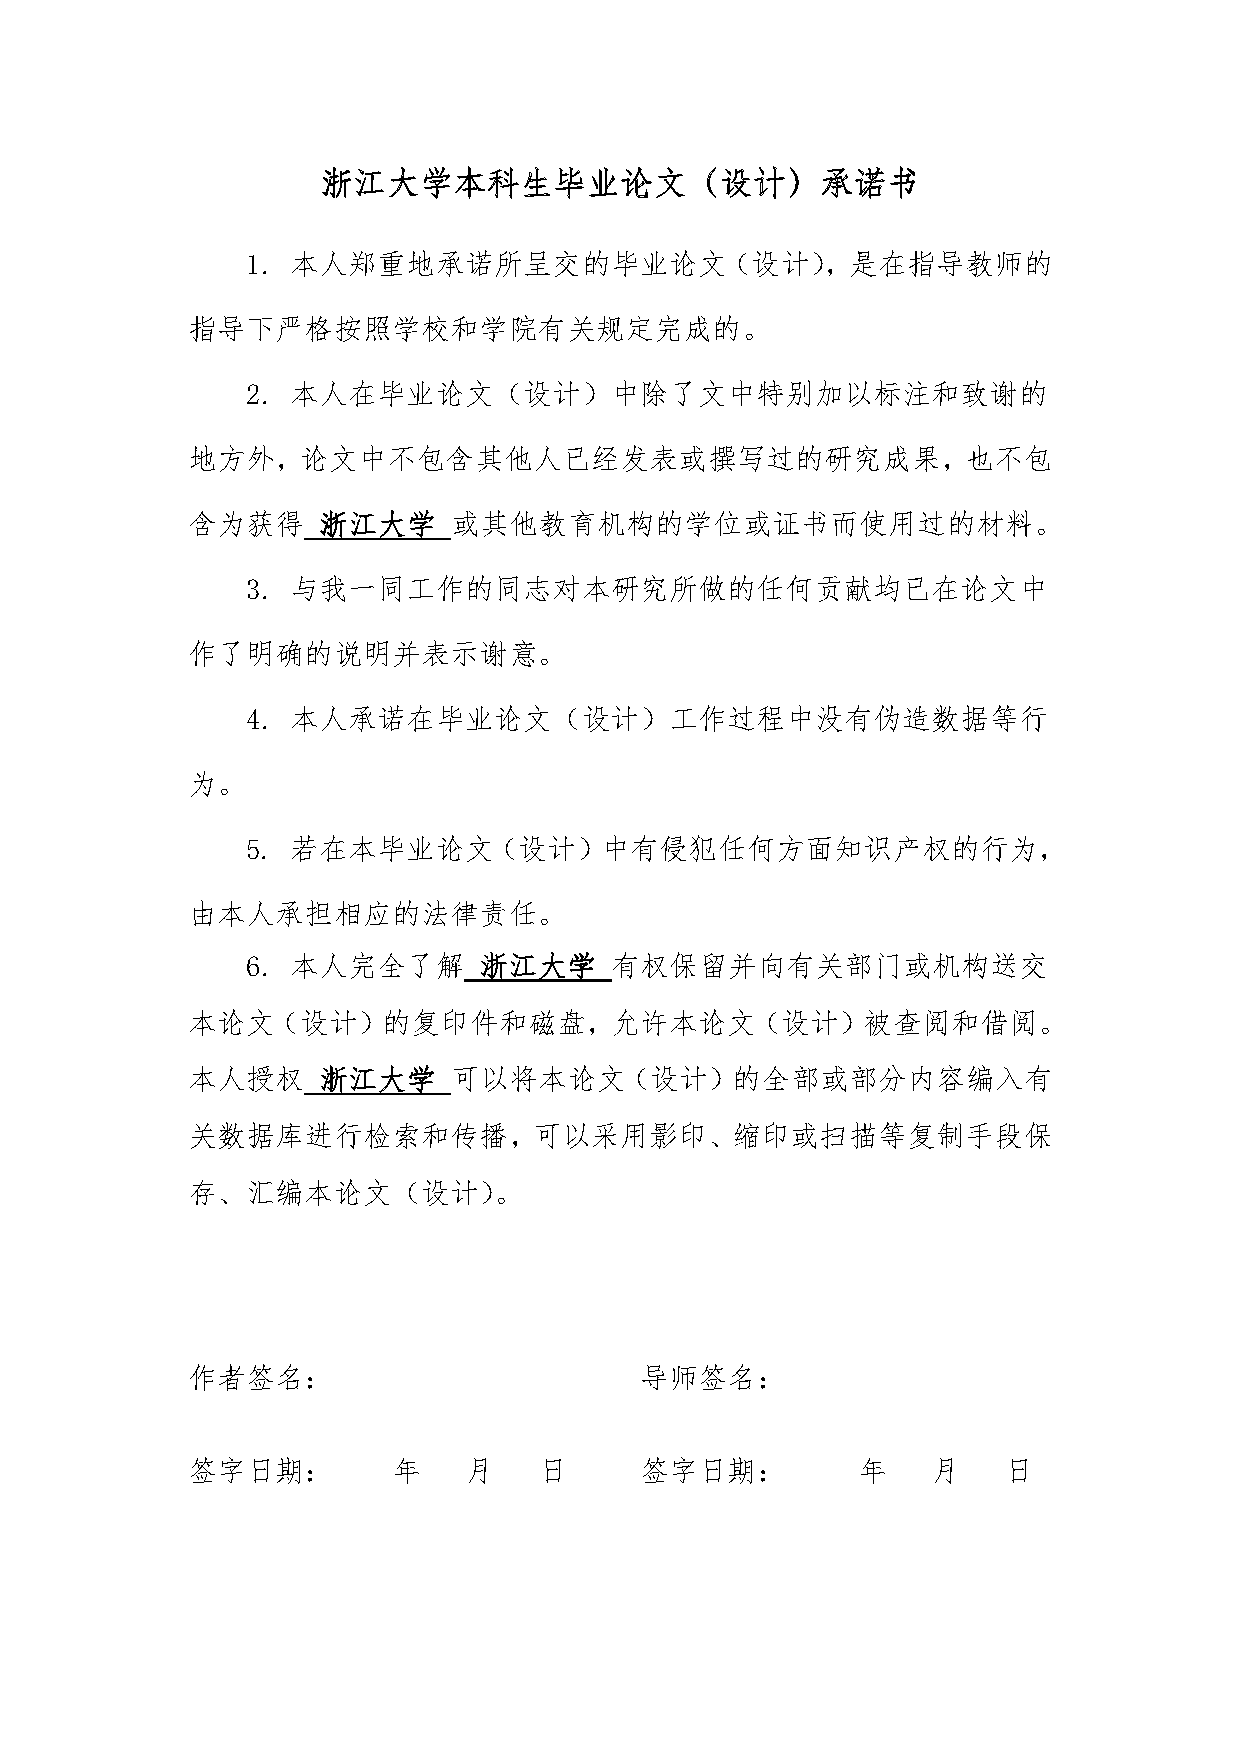
\includepdf[fitpaper=true,pages=-,pagecommand={\chapter*{承诺书}\addcontentsline{toc}{chapter}{承诺书}\thispagestyle{promise}}]{../assets/promise.pdf}
	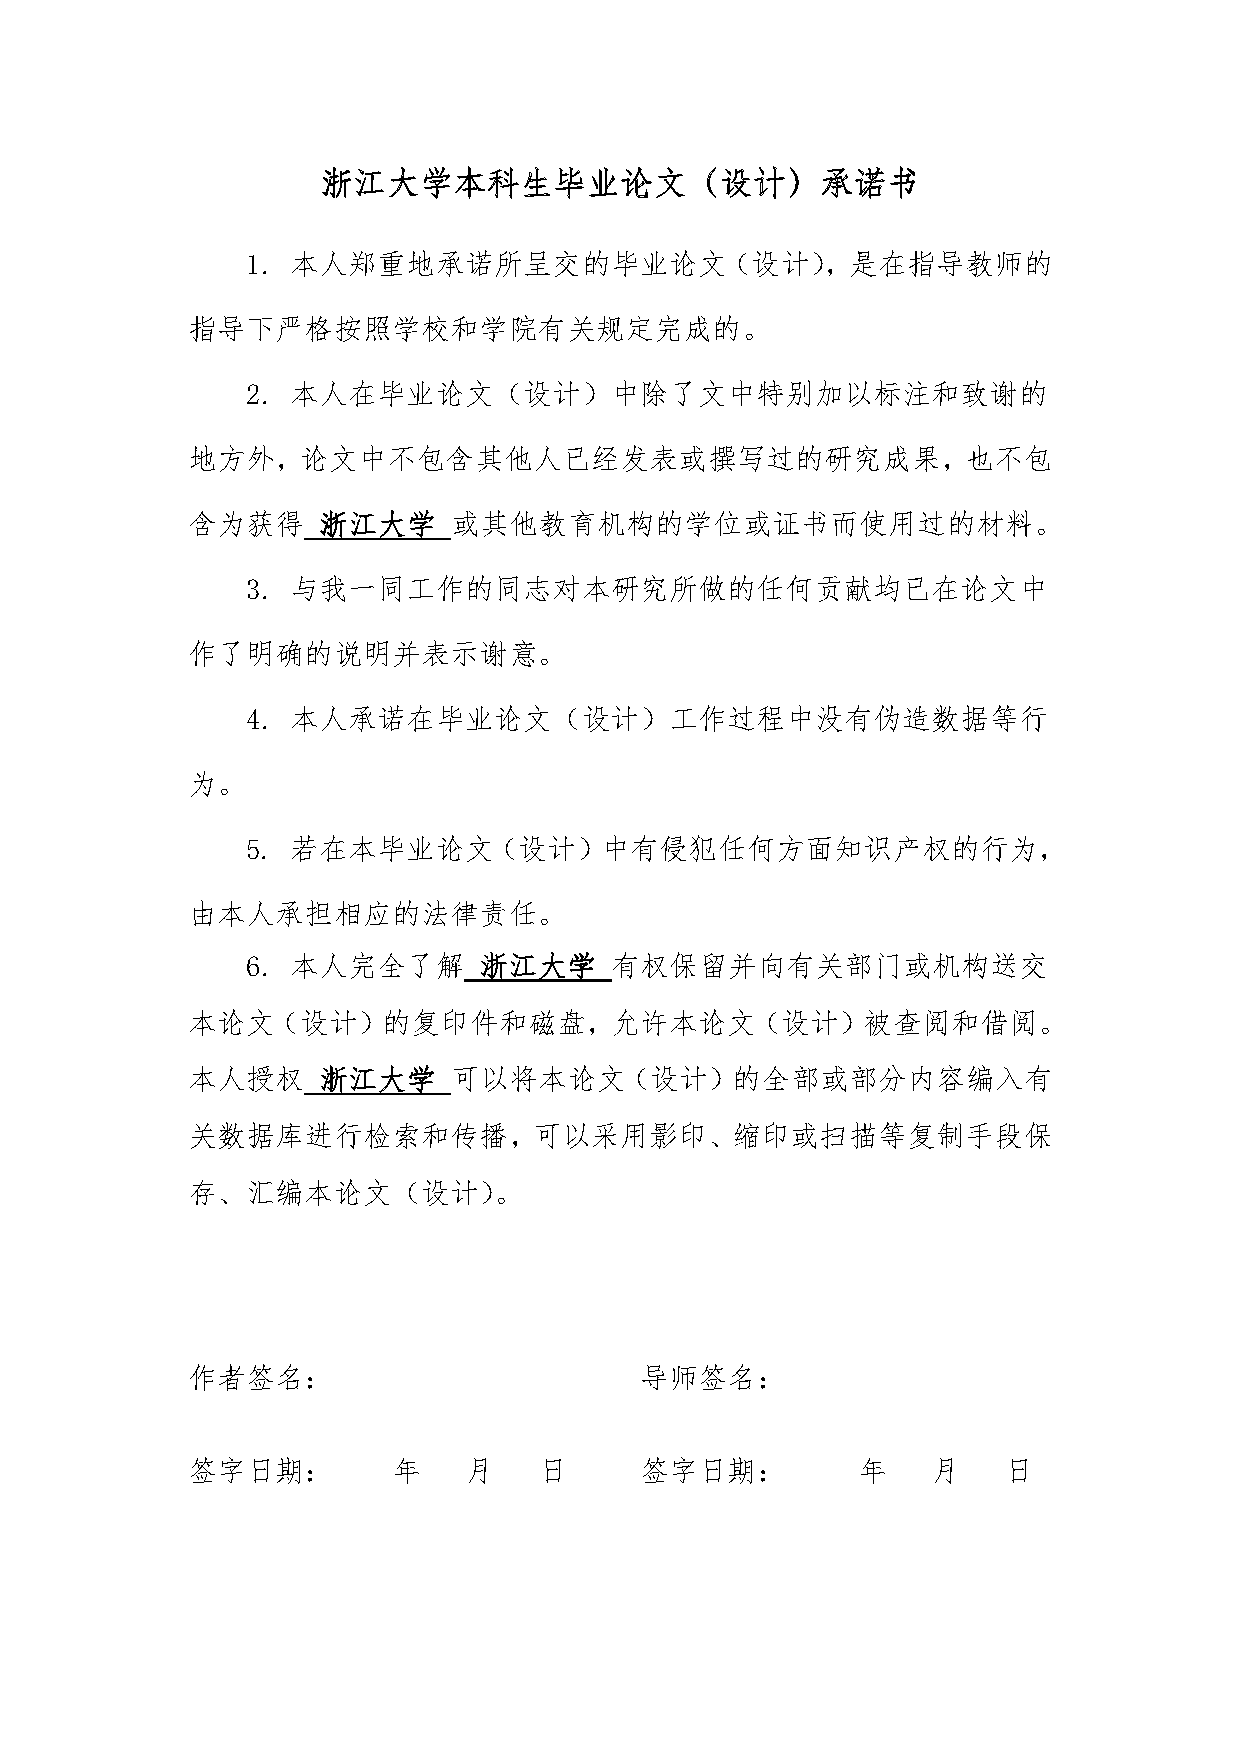
\includepdf[fitpaper=true,pages=-,pagecommand={\thispagestyle{promise}}]{../assets/promise.pdf}
	\begin{acknowledgement}
	谢谢勇于试毒的各位!
	\end{acknowledgement}
	\begin{abstract}
	月色正朦胧,与清风把酒相送...

	\keywords{醉清风,飞蛾扑火}

	\end{abstract}
	\begin{abstract}[en]

	Hello world!

	\keywords{thesis, math}
	\end{abstract}
	
	%\begin{abstract}
月色正朦胧,与清风把酒相送...

\keywords{醉清风,飞蛾扑火}
\end{abstract}
\begin{abstract}[en]
Hello world!

\keywords{thesis, math}
\end{abstract}

    \tableofcontents
	\begin{refsection}
	% part I
% \titleformat{\chapter}
%   {\chap}{\thechapter}{1em}{}
% \titlespacing*{\chapter}{0pt}{3.5ex plus 1ex minus .2ex}{2.3ex plus .2ex}
%
\part{毕业论文(设计)}

\chapter{绪论(章的标题,三号仿宋加黑)}

\begin{equation}
\frac{a}{b}
\end{equation}

\section{节的标题(小三号仿宋加黑)}

\subsection{节的标题(四号仿宋加黑)}

\subsubsection{节的标题,仿宋四号加黑}
\cite{small}
\chapter{正文}

\begin{figure}[H]
    \centering
    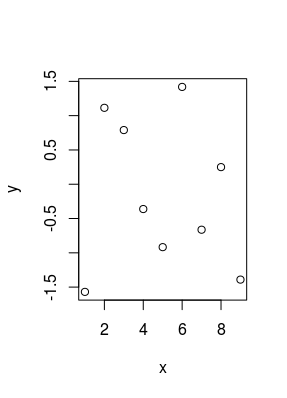
\includegraphics{../assets/sample.png}
    \caption{正态随机数}
\end{figure}

\section{节的标题(仿宋小三号加黑)}
\begin{equation}
\frac{1}{2}
\end{equation}
\subsection{节的标题(仿宋四号加黑)}

符号说明
{\wuhao
\begin{longtable}{p{5cm}p{5cm}}
\caption{符号说明}\\
\hline
项目内容 & 特点\\
\hline
模拟& 同方差\\
\hline
\end{longtable}
}
项目内容

\section{结论}

\printbibliography[heading=chapbib]
	\end{refsection}
	% resume
	\begin{resume}
		【似乎没有明确要求格式,本 demo 提供 enumerate 环境的实现】

		\begin{enumerate}[label=,leftmargin=0em]
		\item 姓名:未雅\quad 性别:未知\quad 民族:未知\quad 出生年月:2000-01-01\quad 籍贯:浙江杭州
		\item 学习经历:
		\begin{enumerate}[label=]
		\item 2000.09-2014.06 学习
		\item 2014.09-2018.06 浙江大学
		\end{enumerate}
		\item 获奖情况:
		\item 参加项目:
		\item 发表的学术论文:
		\end{enumerate}
	\end{resume}
	%\begin{resume}
    【似乎没有明确要求格式,本 demo 提供 enumerate 环境的实现】

    \begin{enumerate}[label=,leftmargin=0em]
    \item 姓名:未雅\quad 性别:未知\quad 民族:未知\quad 出生年月:2000-01-01\quad 籍贯:浙江杭州
    \item 学习经历:
    \begin{enumerate}[label=]
    \item 2000.09-2014.06 学习
    \item 2014.09-2018.06 浙江大学
    \end{enumerate}
    \item 获奖情况:
    \item 参加项目:
    \item 发表的学术论文:
    \end{enumerate}
\end{resume}


	\includepdf[fitpaper=true,pages=-,pagecommand={\thispagestyle{empty}},addtotoc={
		1, alonepage, 1, 《浙江大学本科生毕业论文(设计)任务书》, task
	}]{../assets/official-1-task.pdf}
	\includepdf[fitpaper=true,pages=-,pagecommand={\thispagestyle{empty}},addtotoc={
		1, alonepage, 1, 《浙江大学本科生毕业论文(设计)考核表》,assess
	}]{../assets/official-11-assess.pdf}
	\part{文献综述和开题报告}
	\renewcommand\thechapter{\zhnum{chapter}、} 
	\includepdf[fitpaper= true,pages=-,pagecommand={\thispagestyle{empty}},addtotoc={
		1, alonepage, 1, 文献综述和开题报告封面, cover,
		1, alonepage, 1, 指导教师对文献综述和开题报告具体内容要求, cover,
		1, contabpage, 1, 目录,con,
		1, chapter, 1, 文献综述,s1,
		5, chapter, 1, 开题报告,s2,
		6, chapter, 1, 外文翻译,s3, 
		7, chapter, 1, 外文原文,s4,
		8, alonepage, 1, 《浙江大学本科生文献综述和开题报告考核表》,s5}]{../assets/proposal.pdf}
\end{document}